% VERSTERKER
\section{Opdracht}
    We designen een single-stage common emitter-versterker met werkingsfrequentie $f_0$
    met als centrale NPN-transistor de BFR91A. Voor deze werkingsfrequentie werden
    de $S$-parameters gegeven in \cite{lesWendy}: 
    \[
S = \left[ \begin{array}{cc} 
S_{11} & S_{12} \\ 
 S_{21} & S_{22} \\ 
\end{array} \right] 
 \approx \left[ \begin{array}{cc} 
-0.104 +0.181 j & 0.102 +0.154 j \\ 
1.369 +1.397 j & 0.355 -0.318 j \\ 
\end{array} \right] \label{eq:S}
\]
    
\section{Stabiliteit}
  
    We controleren de nodige en voldoende voorwaarde voor stabiliteit van de versterker door middel van formules 11.71 en 11.72 van \cite{Pozar}.
    \[
      K = \frac{1 - \left| S_{11} \right|^2 - \left| S_{22} \right|^2 + \left| \Delta \right|^2}{2 \left| S_{12}S_{21} \right|} > 1
    \]
    \[
      \left| \Delta \right| < 1
    \]
    \[
      \Delta = \det{S} = S_{11}S_{22} - S_{12}S_{21}
    \]
    
    Aan deze voorwaarden is voldaan, zodat we kunnen besluiten dat de te realiseren versterker onconditioneel stabiel is.
  \section{Stabiliteitscirkels}
    Vermits de versterker onconditioneel stabiel is, zullen de stabiliteitscirkels ofwel de volledige Smith Chart omvatten ofwel buiten de Smith Chart vallen. \tbd{BESPRE CIRKEL = 1}  Met formules 11.68 en 11.69 uit \cite{Pozar}, worden middelpunt $C$ en straal $R$ van de stabiliteitscirkels bepaald.
    \[
      C_L = \frac{\conj{\left(S_{22} - \Delta \conj{S_{11}}\right)}}{\left| S_{22} \right|^2 - \left|\Delta\right|^2}
      \qquad \qquad \qquad
      R_L = \left| \frac{S_{12}S_{21}}{\left| S_{22} \right|^2 - \left|\Delta\right|^2}\right|
    \]
    \[
      C_S = \frac{\conj{\left(S_{11} - \Delta \conj{S_{22}}\right)}}{\left| S_{11} \right|^2 - \left|\Delta\right|^2}
      \qquad \qquad \qquad
      R_S = \left| \frac{S_{12}S_{21}}{\left| S_{11} \right|^2 - \left|\Delta\right|^2}\right|
    \]
    Dit geeft aanleiding tot volgende waarden:
    \[
	C_L =	  2.70 + j   2.15\qquad \qquad \qquad  	R_L =	  2.37
\]

    \[
	C_S =	  7.04  +7.73 j\qquad \qquad \qquad	R_S =	 11.58
\]

    Op figuur \ref{fig:stabCirkels} kunnen deze cirkels ge\"inspecteerd worden.
    \begin{figure}[!h]
      \centering
      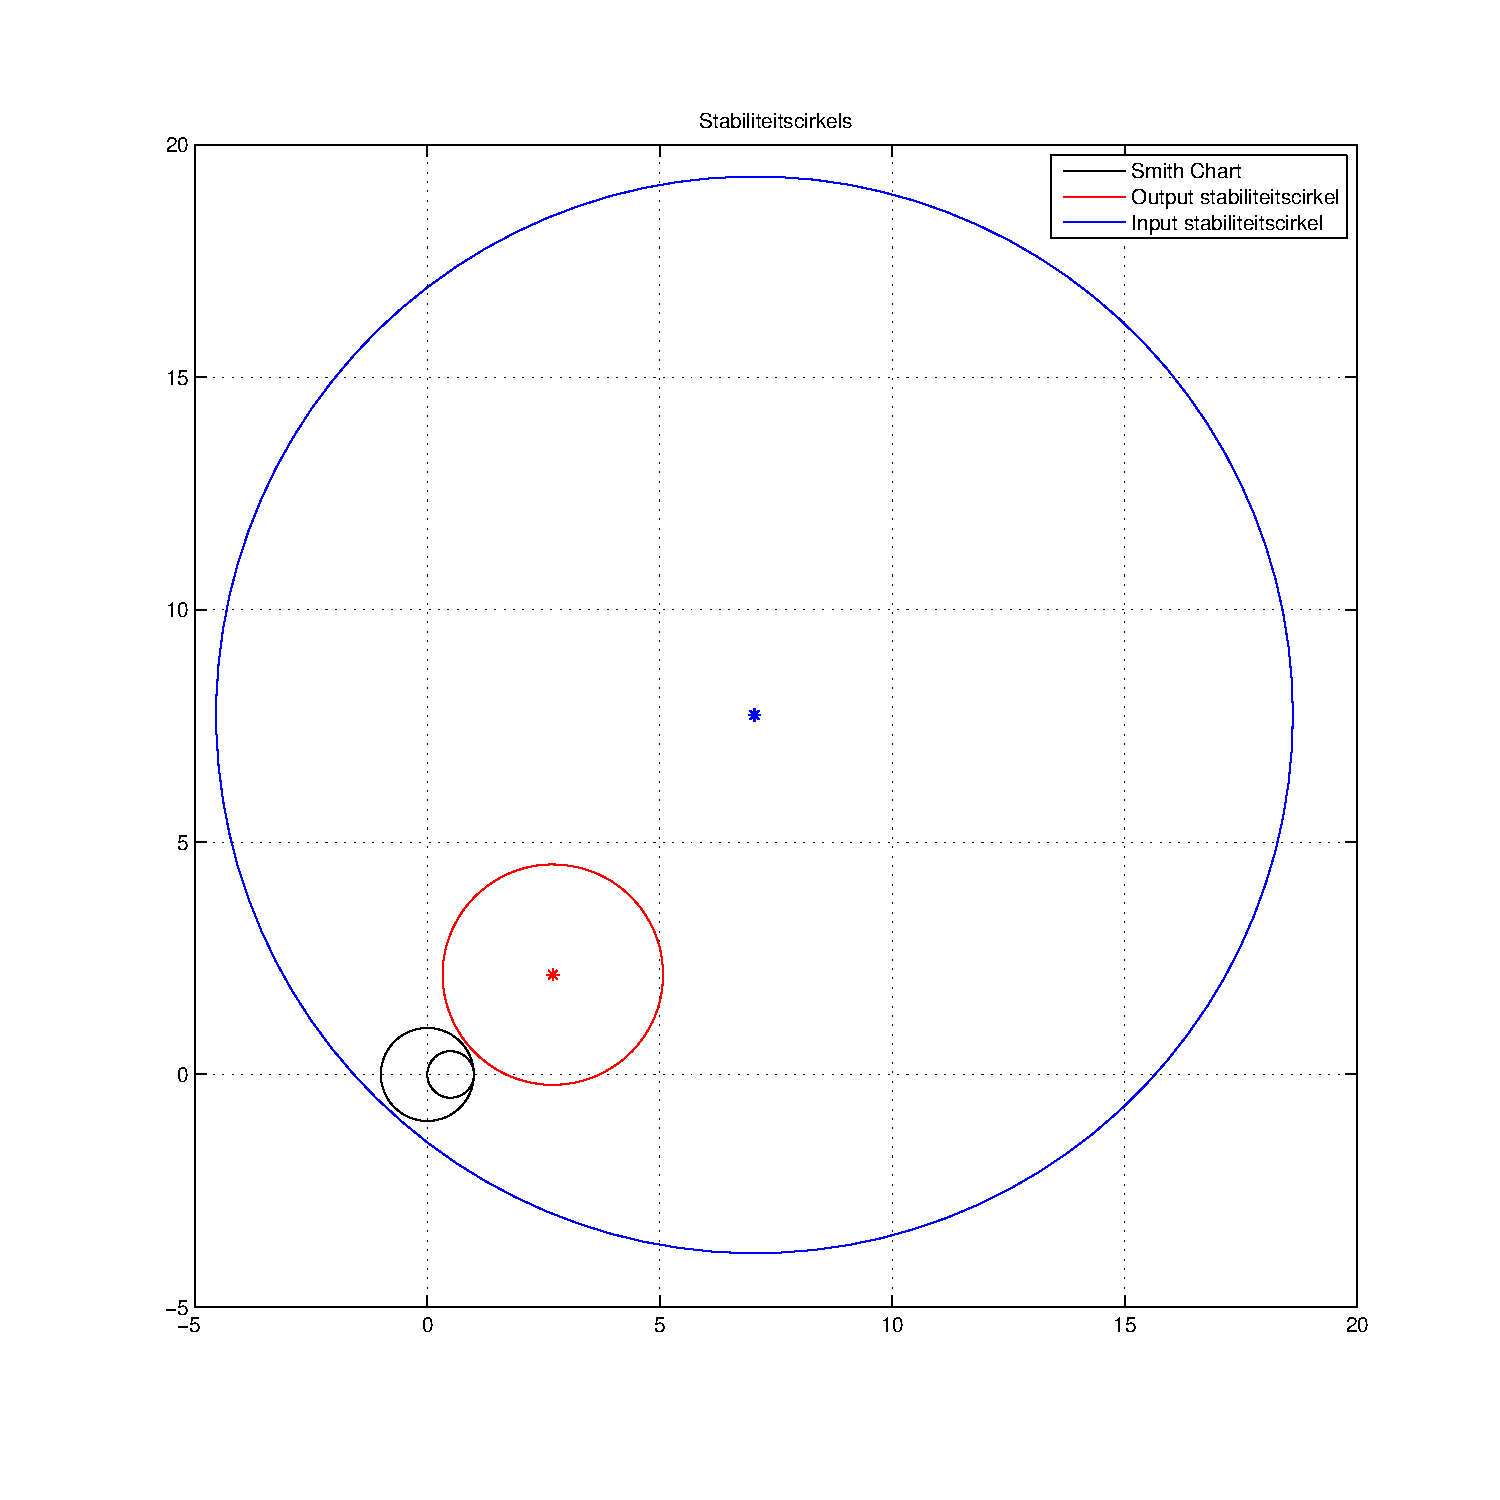
\includegraphics[width=\textwidth,keepaspectratio=true]{fig/stabiliteitscirkels.pdf}  
      \caption{Stabiliteitscirkels} 
      \label{fig:stabCirkels}
    \end{figure}
    Als extra controle, bekijken we welke zones van de Smith Chart stabiel zijn voor input en output. We volgen hier
    een analoge redenering als beschreven op pagina 614 van \cite{Pozar}.
    
    \paragraph{Voor de input} weten we dat indien de output perfect gematcht is ($Z_L = Z_0$ en dus ook $\Gamma_L = 0$, oftewel in het midden van de Smith Chart), we formule 11.62a uit \cite{Pozar}
    \[
      \left| \Gamma_{in} \right| = \left| S_{11} + \frac{S_{12}S_{21}\Gamma_L}{1 - S_{22}\Gamma_L} \right| < 1
    \]
    kunnen vereenvoudigen tot:
    \[
      \left| S_{11} \right|  < 1
    \]
    als voorwaarde voor stabiliteit. Hieraan is voldaan zoals we kunnen zien uit de S-parameters van de transistor. 
    Hierdoor weten we dat het gebied binnen de blauwe inputsstabiliteitcirkel stabiel is.
    
    \paragraph{Voor de output} volgt analoog dat indien de input perfect gematcht is ($Z_S = Z_0$ en dus ook $\Gamma_S = 0$, oftewel in het midden van de Smith Chart), we formule 11.62b uit \cite{Pozar}
    \[
      \left| \Gamma_{out} \right| = \left| S_{22} + \frac{S_{12}S_{21}\Gamma_S}{1 - S_{11}\Gamma_S} \right| < 1
    \]
    kunnen vereenvoudigen tot:
    \[
      \left| S_{22} \right|  < 1
    \]
    als voorwaarde voor stabiliteit. Hieraan is voldaan zoals we kunnen zien uit de S-parameters van de transistor. 
    Hierdoor weten we dat het gebied buiten de rode outputsstabiliteitcirkel stabiel is.
    

\section{Gebruik van de unilaterale benadering}
  Als verantwoording voor de unilaterale benadering, gebruiken we formule 11.86 uit \cite{Pozar} die slechts enkele
  tienden van een dB afwijking mag geven. We nemen hiervoor de grenswaarde van $0.8 dB$
  \[
    -0.8 dB < \frac{1}{\left( 1 + U\right)^ 2} < \frac{G_T}{G_{TU}} < \frac{1}{\left( 1 - U\right)^ 2} < 0.8 dB
  \]
  In deze formule is $U$ de \textit{unilateral figure of merit}:
  \[
    U = \frac{\norm{S_{12}} \norm{S_{21}} \norm{S_{11}} \norm{S_{22}}}{ \left( 1 - \norm{S_{11}}^2 \right) \left( 1 - \norm{S_{22}}^2 \right)}
  \]
  In numerieke waarden, geven deze vergelijkingen dus:
    \[
	U \approx	0.04863
\]
\[
-0.8 \,dB < 0.90940 < \frac{G_T}{G_{TU}} < 1.10484 < 0.8 \,dB
\]
\[
-0.8 dB < -0.825 \,dB< \frac{G_T}{G_{TU}} < 0.866 \,dB< 0.8 \,dB
\]

  Vermits deze ongelijkheden ongeldig zijn, gebruiken we de bilaterale vormen. Maar vermits deze waarden niet te veel afwijken,
  zal een unilaterale benadering geen totaal foute waarden geven.
  
  

\section{Berekening van maximale versterking}
  
  \section{Bepaling van de constante gaincirkels}

\section{Matchingnetwerken}

\section{DC biasnetwerk}

\section{Simulaties}
  \subsection{Ideale transmissielijnen}
  \subsection{Microstrip}

\section{Lay-out}

\section{Metingen}
\subsection{Vergelijking metingen en simulaties}




\tbd{\textbf{Voor het verslag:}
  \begin{itemize}
    \item Alle berekeningen + verwijzing formule
    \item Plots van ideale simulaties + simulatie in microstripversie
    \item Gebruikte Smith Charts voor matching van in- en uitgang
  \end{itemize}
  }